\documentclass{article}

\usepackage{arxiv}

\usepackage[utf8]{inputenc} % allow utf-8 input
\usepackage[T1]{fontenc}    % use 8-bit T1 fonts
\usepackage{hyperref}       % hyperlinks
\usepackage{url}            % simple URL typesetting
\usepackage{booktabs}       % professional-quality tables
\usepackage{amsfonts}       % blackboard math symbols
\usepackage{nicefrac}       % compact symbols for 1/2, etc.
\usepackage{microtype}      % microtypography
\usepackage{lipsum}
\usepackage{graphicx}
\graphicspath{ {./images/} }


\title{Mathematical demonstration of the Multilayer Perceptron and Backpropagation}


\author{
 Rômulo L. Pauliv \\
  %%XX\\
  %%XX\\
  Ponta Grossa, Paraná, Brazil\\
  \texttt{romulopauliv1999@gmail.com} \\
  %% examples of more authors
  %% \AND
  %% Coauthor \\
  %% Affiliation \\
  %% Address \\
  %% \texttt{email} \\
}

\begin{document}
\maketitle
\begin{abstract}
  The aim of this paper is to establish a solid foundation for the mathematical treatment of artificial neural networks in a didactic and clear manner. To achieve this goal, we will mathematically demonstrate the progression from a simple perceptron to the generalization of a multilayer perceptron (MLP), along with the theoretical learning algorithm based on backpropagation.
\end{abstract}


% keywords can be removed
\keywords{ANN \and backpropagation \and ML \and MLP}


\section{Introduction}
As redes neurais artificiais (ANNs) são amplamente reconhecidas por sua eficácia na classificação/reconhecimento de padrões em conjuntos de dados devido à capacidade de aprendizado que possuem. Isso levanta a questão fundamental de como caracterizar o aprendizado em um ambiente não humano e representá-lo de maneira matemática.

Quando falamos em aprendizado, frequentemente o associamos a conceitos como aquisição, retenção e aplicação de informações em diferentes contextos. No entanto, uma análise mais profunda nos leva a relacionar o aprendizado com o conceito de erro e processos iterativos. 

Tal fator se deve à constatação de que, ao agir sobre algum objeto com a intenção de gerar um resultado específico sem ter ciência de que maneira, estamos expostos a falhar nesse objetivo. Executando a ação inúmeras vezes, é possível encontrar a ação que gera a resultante específica desejada, onde, ao encontrá-la, podemos discernir as ações que levam ou não a resultante esperada. Logo, podemos conceber que um dos resultados do aprendizado é a capacidade de discernir se algo está em desacordo com a realidade já observada, ou seja, um erro. 

Nesse contexto, é necessário julgar tal objeto com base em suas propriedades observadas para atribuir diferentes estados a ele e, caso esse estado esteja em desacordo com a realidade já observada, é necessário o ajuste da ação julgar. Portanto, se atribuímos a capacidade de aprendizado a um objeto, esse objeto também deve ser capaz de atribuir diferentes estados a outros objetos com base na sua percepção, ajustando constantemente o mecanismo que faz tal atribuição. 

Para isso, Frank Rosenblatt cunhou o termo "perceptron" em seu trabalho "Principles of Neurodynamics: Perceptrons and the Theory of Brain Mechanisms". Assim, iniciaremos nossa abordagem matemática das ANNs com o desenvolvimento de um objeto elementar dotado de percepção, ou seja, o perceptron. Após, iremos aprovisionar tal percetron de maior complexidade com o objetivo de capacitá-lo em gerir e correlacionar mais informações, isto é, um multilayer percetron (MLP). Por último, dotá-lo com a capacidade de julgamento através de sua percepção. 



\section{Perceptron}
Nosso objetivo é construir um perceptron que seja descrito por uma função \(f\) tal que \(f: \mathbb{R}^n \rightarrow \Theta\) onde \(\Theta\) representa qualquer contradomínío possível. Isso implica que, nessa função as variáveis independentes ou inputs representarão o estímulo do perceptron e a variável dependente ou output a resposta desse estímulo. 

\subsection[]{Inputs}

O input será denotado por um vetor \(X\) tal que \(X \in \mathbb{R}^n\). Logo, temos que \(X^T = [x_1, \dots, x_n]\) onde o superescrito \(T\) representa a forma transposta do vetor \(X\). Repare que no vetor não há o elemento \(x_0\). Isso se deve ao fato que iremos reservar tal termo para o que futuramente será introduzido como o bias. Logo, os inputs ou variáveis independentes serão listado de \(i=1, \dots, n\).

\subsection[]{Outputs}

O output será denotado por um vetor \(Y\) tal que \(Y \in \Theta\). Logo, temos que \(Y = [y_1]\). No output não haverá a adição do bias futuramente mas evitaremos utilizar o índice zero para evitar enganos futuros. O domínio \(\Theta\) representa qualquer domínimo possível tal que \(\Theta\) será ditado pela função de ativação que iremos introduzir em breve. No perceptron teremos o vetor \(Y\) com apenas uma dimensão. Futuramente iremos introduzir um vetor de saída com \(m\)-outputs. Logo, os outputs ou variáveis dependentes serão listado de \(i=1, \dots, m\).

\subsection[]{Weights}
Os pesos serão parte substancial de nosso perceptron. Tais pesos irão transformar nossos \(n\)-inputs a fim de resultar em elementos de \(Y\). Logo, os pesos serão denotados por \(\varpi\) tal que \(\varpi \in \mathbb{R}^n\). 


\subsection{Headings: second level}
\lipsum[5]
\begin{equation}
  \xi _{ij}(t)=P(x_{t}=i,x_{t+1}=j|y,v,w;\theta)= {\frac {\alpha _{i}(t)a^{w_t}_{ij}\beta _{j}(t+1)b^{v_{t+1}}_{j}(y_{t+1})}{\sum _{i=1}^{N} \sum _{j=1}^{N} \alpha _{i}(t)a^{w_t}_{ij}\beta _{j}(t+1)b^{v_{t+1}}_{j}(y_{t+1})}}
\end{equation}

\subsubsection{Headings: third level}
\lipsum[6]

\paragraph{Paragraph}
\lipsum[7]

\section{Examples of citations, figures, tables, references}
\label{sec:others}
\lipsum[8] \cite{kour2014real,kour2014fast} and see \cite{hadash2018estimate}.

The documentation for \verb+natbib+ may be found at
\begin{center}
  \url{http://mirrors.ctan.org/macros/latex/contrib/natbib/natnotes.pdf}
\end{center}
Of note is the command \verb+\citet+, which produces citations
appropriate for use in inline text.  For example,
\begin{verbatim}
   \citet{hasselmo} investigated\dots
\end{verbatim}
produces
\begin{quote}
  Hasselmo, et al.\ (1995) investigated\dots
\end{quote}

\begin{center}
  \url{https://www.ctan.org/pkg/booktabs}
\end{center}


\subsection{Figures}
\lipsum[10]
See Figure \ref{fig:fig1}. Here is how you add footnotes. \footnote{Sample of the first footnote.}
\lipsum[11]

\begin{figure}
  \centering
  \fbox{\rule[-.5cm]{4cm}{4cm} \rule[-.5cm]{4cm}{0cm}}
  \caption{Sample figure caption.}
  \label{fig:fig1}
\end{figure}

\begin{figure} % picture
  \centering
  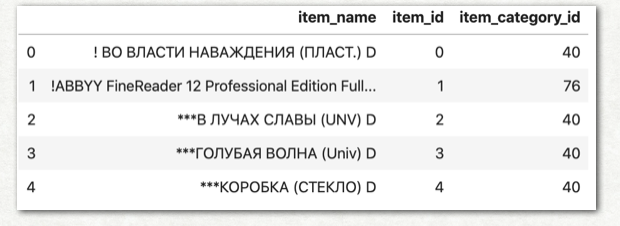
\includegraphics{test.png}
\end{figure}

\subsection{Tables}
\lipsum[12]
See awesome Table~\ref{tab:table}.

\begin{table}
  \caption{Sample table title}
  \centering
  \begin{tabular}{lll}
    \toprule
    \multicolumn{2}{c}{Part}                   \\
    \cmidrule(r){1-2}
    Name     & Description     & Size ($\mu$m) \\
    \midrule
    Dendrite & Input terminal  & $\sim$100     \\
    Axon     & Output terminal & $\sim$10      \\
    Soma     & Cell body       & up to $10^6$  \\
    \bottomrule
  \end{tabular}
  \label{tab:table}
\end{table}

\subsection{Lists}
\begin{itemize}
  \item Lorem ipsum dolor sit amet
  \item consectetur adipiscing elit.
  \item Aliquam dignissim blandit est, in dictum tortor gravida eget. In ac rutrum magna.
\end{itemize}


\bibliographystyle{unsrt}
%\bibliography{references}  %%% Remove comment to use the external .bib file (using bibtex).
%%% and comment out the ``thebibliography'' section.


%%% Comment out this section when you \bibliography{references} is enabled.
\begin{thebibliography}{1}

  \bibitem{kour2014real}
  George Kour and Raid Saabne.
  \newblock Real-time segmentation of on-line handwritten arabic script.
  \newblock In {\em Frontiers in Handwriting Recognition (ICFHR), 2014 14th
      International Conference on}, pages 417--422. IEEE, 2014.

  \bibitem{kour2014fast}
  George Kour and Raid Saabne.
  \newblock Fast classification of handwritten on-line arabic characters.
  \newblock In {\em Soft Computing and Pattern Recognition (SoCPaR), 2014 6th
      International Conference of}, pages 312--318. IEEE, 2014.

  \bibitem{hadash2018estimate}
  Guy Hadash, Einat Kermany, Boaz Carmeli, Ofer Lavi, George Kour, and Alon
  Jacovi.
  \newblock Estimate and replace: A novel approach to integrating deep neural
  networks with existing applications.
  \newblock {\em arXiv preprint arXiv:1804.09028}, 2018.

\end{thebibliography}


\end{document}
